%iffalse
\let\negmedspace\undefined
\let\negthickspace\undefined
\documentclass[journal,12pt,onecolumn]{IEEEtran}
\usepackage[version=4]{mhchem}
\usepackage{chemformula} % for \ch if needed
\usepackage{chemfig}
\usepackage{chemmacros}
\chemsetup{modules = reactions} % Enables reaction arrows
\usepackage{graphicx}
\graphicspath{ {./images/} }
\usepackage{geometry}
\usepackage{lastpage}
\usepackage{cite}
\usepackage{amsmath,amssymb,amsfonts,amsthm}
\usepackage{enumitem,multicol}
\usepackage{algorithmic}
\usepackage{graphicx}
\usepackage{textcomp}
\usepackage{xcolor}
\usepackage{txfonts}
\usepackage{listings}
\usepackage{enumitem}
\usepackage{mathtools}
\usepackage{gensymb}
\usepackage{comment}
\usepackage[breaklinks=true]{hyperref}
\usepackage{tkz-euclide} 
\usepackage{listings}
\usepackage{gvv}                                        
%\def\inputGnumericTable{}                                 
\usepackage[latin1]{inputenc}                                
\usepackage{color}                                            
\usepackage{array}                                            
\usepackage{longtable}                                       
\usepackage{calc}                                             
\usepackage{multirow}                                         
\usepackage{hhline}                                           
\usepackage{ifthen}                                           
\usepackage{lscape}
\usepackage{tabularx}
\usepackage{array}
\usepackage{float}


\newtheorem{theorem}{Theorem}[section]
\newtheorem{problem}{Problem}
\newtheorem{proposition}{Proposition}[section]
\newtheorem{lemma}{Lemma}[section]
\newtheorem{corollary}[theorem]{Corollary}
\newtheorem{example}{Example}[section]
\newtheorem{definition}[problem]{Definition}
\newcommand{\BEQA}{\begin{eqnarray}}
\newcommand{\EEQA}{\end{eqnarray}}
\newcommand{\define}{\stackrel{\triangle}{=}}
\theoremstyle{remark}

\geometry{margin=1 in}



\setlength{\headheight}{14pt}
\setlength{\headsep}{5pt}
\setlength{\footskip}{20pt}



\begin{document}
\begin{enumerate}
    



\item
If a complex variable 
\[
z = \frac{\sqrt{3}}{2} + \frac{i}{2},
\]
then \( z^4 \) is
\hfill{GATE 2007 PI}
\begin{enumerate}
\begin{multicols}{4}
\item $2\sqrt{3} + i \cdot 2$
\item $-\frac{1}{2} + i \frac{\sqrt{3}}{2}$
\item $\frac{\sqrt{3}}{2} - i \frac{1}{2}$
\item $\frac{\sqrt{3}}{8} + i \frac{1}{8}$
\end{multicols}
\end{enumerate}



    
    
    
  \item 
    Two cards are drawn at random in succession,with replacement, from a deck of 52 well shuffled cards. Probability of getting both 'Aces' is
    \hfill{GATE 2007 PI}
    \begin{enumerate}
    \begin{multicols}{4}
        \item 1/169
        \item 2/169
        \item 1/13
        \item 2/13
        \end{multicols}
    \end{enumerate}
    
    \item 
    The angle(in degrees)between two planar vectors 
    
$\vec{a} = \frac{\sqrt{3}}{2} \, i + \frac{1}{2} \, j$
and $\vec{b} = -\frac{\sqrt{3}}{2} \, i + \frac{1}{2} \, j$

      is
      \hfill{GATE 2007 PI}
      \begin{enumerate}
      \begin{multicols}{4}
          \item 30
          \item 60
          \item 90
          \item 120
          \end{multicols}
      \end{enumerate}
      
      \item 
        What is the value of
\begin{figure}[H]
    \centering
    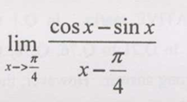
\includegraphics[width=0.25\linewidth]{figs/Q.4.png}
    \caption{fig1}
    \label{figs:figs/Q.4.png}
\end{figure}
\hfill{GATE 2007 PI}
\begin{enumerate}
\begin{multicols}{4}
    \item $\sqrt{2}$
    \item 0
    \item $-\sqrt{2}$
    \item Limit does not exist
    \end{multicols}
     \end{enumerate} 
    
    \item 
    The determinant
\[
\begin{vmatrix}
1+b & b & 1 \\
b & 1+b & 1 \\
1 & 2b & 1
\end{vmatrix}
\]

evaluates to
\hfill{GATE 2007 PI}
\begin{enumerate}
\begin{multicols}{4}
    \item 0
    \item 2b(b-1)
    \item 2(1-b)(1+2b)
    \item 3b(1+b)
    \end{multicols}
\end{enumerate}

\item 
f(x) =$|x|$ is a function defined for real numbers x.The directional derivative of f at x=o in the direction d=-1 is
\hfill{GATE AI 2025}
\begin{enumerate}
\begin{multicols}{4}
    \item 1
    \item 0
    \item -1/2
    \item -1
    \end{multicols}
\end{enumerate}

\item 
Whixh one of the following planar mechanisms does NOT provide quick-return motion?

\hfill{GATE 2007 PI}
\begin{enumerate}
\begin{multicols}{2}
    

    \item Scotch-Yoke
    \item Whitworth
    \item Off-set slider crank
    \item Drag link
    \end{multicols}
    \end{enumerate}
    
    \item 
    The geometric tolerance that does NOT a datum for its specification is 
    \hfill{GATE 2007 PI}
    \begin{enumerate}
    \begin{multicols}{4}
        \item Concentricity
        \item Runout
        \item Perpendicularity
        \item Flatness
        \end{multicols}
    \end{enumerate}
    
    \item 
    Oil in hydraolic cylinder is compressed from an intial volume of 2 $m^3$ to 1.96 $m^3$.If the pressure of oil in the cylinder changes from 40 MPa to 80 MPa during compression, the bulk modulus of elasticity of oil is
    \hfill{GATE 2007 PI}
    
    \begin{enumerate}
    \begin{multicols}{4}
        \item 1000 MPa
        \item 2000 MPa
        \item 4000 MPa
        \item 8000 MPa
        \end{multicols}
    \end{enumerate}
    
    \item 
    A component of a material with a modulus of elasticity of 200 MPa and modulus of rigidity 80 MPa experiences an axial strain of 1000. The lateral strain experienced by the component within the elastic limit is
    
    \hfill{GATE 2007 PI}
    \begin{enumerate}
    \begin{multicols}{4}
        \item 250
        \item 400
        \item 500
        \item 800
        \end{multicols}
    \end{enumerate}
    
    \item
    Which one of the folowing cooling methods is best suited for converting Austetine steel into very fine Pearlite steel?
    \hfill{GATE 2007 PI} 
    \begin{enumerate}
    \begin{multicols}{4}
        \item Oil quenching
        \item Water quenching
        \item Air cooling
        \item Furnace cooling
        \end{multicols}
        \end{enumerate}
        
        \item
        Reaming is primarly used for achieving
        \hfill{GATE 2007 PI}
        \begin{enumerate}
        \begin{multicols}{2}
            \item Higher MRR
            \item Improved dimensional tolerance
            \item Fine surface finish
            \item Improved positional tolerance
            \end{multicols}
        \end{enumerate}
        
        \item 
        The interpolator in a CNC machine controls
        \hfill{GATE 2007 PI}
        \begin{enumerate}
        \begin{multicols}{4}
            \item Sindle speed
            \item Coolant flow
            \item Feed rate
            \item Tool change
            \end{multicols}
        \end{enumerate}
        
        \item 
        Which one of the following instruments is a comparator?
        \hfill{GATE 2007 PI}
        \begin{enumerate}
        \begin{multicols}{4}
            \item Tool Maker's Microscope
            \item GO/NO GO gage
            \item Optical Interferometer
            \item Dial Gauge
            \end{multicols}
        \end{enumerate}
        
        \item 
        Which one of the following is a indispensable part of just-in-Time manufacturing of multiple products on a line?
        \hfill{GATE 2007 PI}
        \begin{enumerate}
        \begin{multicols}{2}
            \item Outbiund quality inspection
            \item Lot sizing
            \item Safety stocks
            \item Set up time reduction
            \end{multicols}
        \end{enumerate}
    
        \item 
       	During an economic analysis of a capital investment proposal, the cost that can be ignored is


        \hfill{GATE 2007 PI}
        \begin{enumerate}
        \begin{multicols}{4}
            \item Sunk cost
            \item Fixed cost
            \item Marginal cost
            \item Variable cost
            \end{multicols}
            \end{enumerate}
            
            \item 
            	Which one of the following is an effective therblig?
            \hfill{GATE 2007 PI}
            \begin{enumerate}
            \begin{multicols}{4}
                \item Position
                \item Inspect
                \item Grasp
                \item Search
                \end{multicols}
            \end{enumerate}
            
            \item 
            In queueing models, M/M/c denotes a Poisson arrival process and
            \hfill{GATE 2007 PI}
            \begin{enumerate}
            \begin{multicols}{2}
                \item 	exponentially distributed service times and c servers in series
                \item 	constant service times and c servers in series
                \item 	exponentially distributed service times and c servers in parallel
                \item 	exponentially distributed service times and c servers in parallel
                \end{multicols}
            \end{enumerate}
            
            \item 
            A product is made by mixing three raw materials l , 2, 3 in varying proportions, where material I must account for not more than 50\% of the total.If x,y and z are the amounts of raw materials 1,2,3 respectively,this constant can be modeled as
            \hfill{GATE 2007 PI}
            \begin{enumerate}
            \begin{multicols}{4}
                \item $x \leq 0.5$
                \item $x \leq 0.5(x+y+z) $
                \item $0.5x \leq x+y+z $
                \item $x \geq 0.5(y+z) $
                \end{multicols}
            \end{enumerate}
            
        
            \item 
            Which one of the following cost components is a part of appraisal costs related to quality


            \hfill{GATE 2007 PI}
            \begin{enumerate}
            \begin{multicols}{4}
                \item Quality planning and engineering cost
                \item Process control cost
                \item Quality data acquisition and analysis cost
                \item Product inspection and testing cost
                \end{multicols}
\end{enumerate}
{Q. 21 to Q. 75 carry two marks each.}



\item
If X is a continuous random variable whose probability density function is given by
       \[
f(x) =
\begin{cases}
K(5x - 2x^2), & 0 \leq x \leq 2, \\
0, & \text{otherwise}.
\end{cases}
\]
 Then P(X>1) is
        
        
        
            is
            \hfill{GATE 2007 PI}
            \begin{enumerate}
            \begin{multicols}{4}
                \item 3/14
                \item 4/5
                \item 14/17
                \item 17/28
                \end{multicols}
            \end{enumerate}
            
            \item 
            The random variable X takes on the values l , 2, or 3 with probabilities (2+5P)/5,(1+3P)/5, and (1.5+2P)/5,respectively.The values of P and E[X] are respectively
\hfill{GATE 2007 PI}

            \begin{enumerate}
            \begin{multicols}{4}
                \item 0.05,1.87
                \item 1.90,5.87
                \item 0.05,1.10
                \item 0.25,1.40
                \end{multicols}
            \end{enumerate}
            
            \item
           	If A is square symmetric real valued matrix of dimension 2n. the eigensalues of A are


            \hfill{GATE 2007 PI}
            \begin{enumerate}
            \begin{multicols}{2}
                \item 2n distinct real values 
                \item 	2n real values, not necessarily distinct
                \item 	n distinctpairs of complex conjugate numbers
                \item n pairs of complex conjugate numbers. not necessarily distinct
                \end{multicols}
            \end{enumerate}
        
           \item
            The function $e^{x}$ over the interval [0,1] is to be evaluated using the Taylor series 1+x+$\frac{x^{2}}{2!}$+$\frac{x^{3}}{3!}$+... to accuracy of $\delta>0$.The number of terms in the series that is considered for this accuracy is n. Then


            \hfill{GATE 2007 PI}
            \begin{enumerate}
            \begin{multicols}{2}
                \item for a given $x \in [0,1]$ and a given $\delta$, there is no finite n that is valid
                 \item for a given $\delta > 0$, there is a valid n that is finite for a given $x \in[0,1] $, but there is no finite n that is valid for all $x \in[0,1]$
                 \item for a given $\delta >0$,there is a finite n that is valid for all $x \in [0,1]$
                 \item there is a finite n that is valid for all x in [0,1] an all $\delta >0$
                 \end{multicols}
                 \end{enumerate}
            
            \item 
                 for the function f(x,y)=$x^{2}$ -$y^{2}$ defined as $R^{2}$ ,The point [0,0] is
                 \hfill{GATE 2007 PI}
                 \begin{enumerate}
                 \begin{multicols}{4}
                \item a local minimum
                \item a local maximum
                \item neither a local minimum nor a local    maximum
                \item both a local maximum and a local minimum
                \end{multicols}
                 \end{enumerate}

\item
$q_{1}$,.....$q_{m}$ are n-dimensional vectors , with $m < n$. This set of vectors is linearly dependent. Q is the matrix with $q_{1}$,.....$q_{m}$ as the columns. The rank of Q is
\hfill{GATE 2007 PI}
\begin{enumerate}
\begin{multicols}{4}
    \item Less than m
    \item m
    \item between m and n
    \item n
    \end{multicols}
    \end{enumerate}
    
    \item 
    "Matching Exercise". Choose the correct one out of the alternatives A,B,C,D
   
        \begin{tabular}{c|c}
        Group 1     &  Group 2\\
      P-Second order differential equations       & 1-Runge-Kutta method\\
      Q-Nonlinear algebraic equations & 2-Newton-Raphson method\\
      R-Linear algebraic equations & 3-Gauss elimination\\
      S-Numerical integration & 4-Simpson's rule
      
        \end{tabular}
        \hfill{GATE 2007 PI}
        \begin{enumerate}
        \begin{multicols}{2}
            \item P-3,Q-2,R-4,S-1
            \item P-2,Q-4,R-3,S-1
            \item P-1,Q-2,R-3,S-4
            \item P-1,Q-3,R-2,S-4
            \end{multicols}
        \end{enumerate}
        
       \item 
        	A disc type flywheel having a mass of 10 kg and radius 0.2 m is replaced in a single cylinder engine by a system of dynamically equivalent concentrated masses $m_{1}$ and $m_{2}$ rotating about the flywheel axis as shown below. If the distance $x_{1}$ is 0.1 m then the distance $x_{2}$ is
            
             
                  \begin{figure}[H]
                      \centering
                      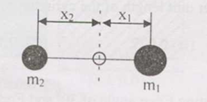
\includegraphics[width=0.3\linewidth]{figs/Q.28.png}
                      \caption{fig2}
                      \label{fig:figs/Q.28.png}
                  \end{figure}
                  
                \hfill{GATE 2007 PI}
                \begin{enumerate}
                \begin{multicols}{4}
                    \item 0.1 m
                    \item 0.2 m
                    \item 0.4 m
                    \item 0.8 m
                    \end{multicols}
                    \end{enumerate}
                    
                    \item 
                    A radial disc cam rotating at a constant speed of 60 rpm provides a parabolic displacement of 0.2 m to its fiat faced rectilinear follower during 900 of its rotation. The acceleration (m/s-) experienced by the follower is
                    \hfill{GATE 2007 PI}
                    \begin{enumerate}
                    \begin{multicols}{4}
                        \item 0.8
                        \item 1.6
                        \item 3.2
                        \item 6.4
                        \end{multicols}
                    \end{enumerate}
                    
                    \item
                    Figure below shows a mass of 300 kg being pushed using a cylindrical rod made of a material having E = 22 MPa arid of 2 m length and 0.1 m in diameter. In order to avoid the failure of the rod due to elastic instability, the maximum value of the coefficient of Coulomb friction permissible between the mass and the floor is

    \begin{figure}[H]
        \centering
        
\includegraphics[width=0.5\linewidth]{figs/Q.30.png}
        \caption{fig3}
        \label{fig:figs/Q.30.png}
    \end{figure}
                   \hfill{GATE 2007 PI}
\begin{enumerate}
\begin{multicols}{4}
    \item 0.22
    \item 0.36
    \item 0.65
    \item 0.75
    \end{multicols}
\end{enumerate}

\item
A cylindrical tank is filled with water as shown in the Figure below. The force required to close the discharge tube at the bottom of the tank is

\begin{figure}[H]
    \centering
    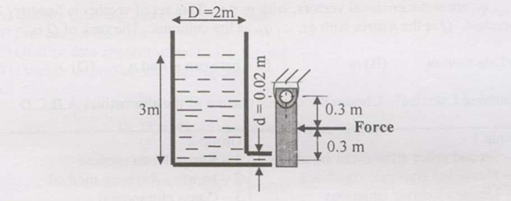
\includegraphics[width=0.5\linewidth]{figs/Q.31.png}
    \caption{fig4}
    \label{fig:figs/Q.31.png}
\end{figure}


 \hfill{GATE 2007 PI}
 \begin{enumerate}
 \begin{multicols}{4}
     \item 18.5 N
     \item 37 N
     \item 45.5 N
     \item 74 N
     \end{multicols}
 \end{enumerate}

 \item
 When an ideal gas (Cp = 3.5) is heated at constant pressure from $25^\circ\mathrm{C}$
 to $425^\circ\mathrm{C}$
, the change in entropy is
\hfill{GATE 2007 PI}
\begin{enumerate}
\begin{multicols}{4}
    \item 1.48
    \item 2.97
    \item 4.2
    \item 5.98
    \end{multicols}
\end{enumerate}

\item
A long glass cylinder of inner diameter = 0.03 m and outer diameter = 0.05 m carries' hot fluid inside. If the thermal conductivity of glass = 1.05 W/mK, the thermal resistance ($^\circ\mathrm{K}\!/\mathrm{W}$
) per unit length of the cylinder is
\hfill{GATE 2007 PI}
\begin{enumerate}
\begin{multicols}{4}
    \item 0.031
    \item 0.077
    \item 0.17
    \item 0.34
    \end{multicols}
\end{enumerate}

\item
	A tool with Side Cutting Edge angle of $30^\circ\mathrm{C}$
 and End Cutting Edge angle of $10^\circ\mathrm{C}$
 is used for fine turning with a feed of 1 mm/rev. Neglecting nose radius of the tool, the maximum (peak to valley) height of surface roughness produced will be
 \hfill{GATE 2007 PI}
 \begin{enumerate}
 \begin{multicols}{4}
     \item 0.16 mm
     \item 0.26 mm
     \item 0.32 mm
     \item 0.48 mm
     \end{multicols}
      \end{enumerate}
      
      \item
	Which one of the following process conditions leads to higher MRR in ECM process?
    
    \hfill{GATE 2007 PI}
    \begin{enumerate}
    \begin{multicols}{2}
        \item higher current, larger atomic weight
        \item higher valency, lower current
        \item ) lower atomic weight, lower valency 
        \item higher valency, lower atomic weight
        \end{multicols}
    \end{enumerate}
    
    \item
     In an Abrasive Jet Machining process, if Q = flow rate of the abrasives and d = the mean diameter of the abrasive grain, then material removal rate is proportional to
     \hfill{GATE 2007 PI}
     \begin{enumerate}
     \begin{multicols}{4}
         \item $\frac{Q}{d^2}$
         \item Qd
         \item $Qd^2$
         \item $Qd^3$
         \end{multicols}
\end{enumerate}

\item
"Matching Exercise". Choose the correct one out of the alternatives A, B, C, D

   \begin{tabular}{c|c}
   Group 1      &  Group 2\\
P-Plastic Carry-Bags         & 1-Theramal-Vacuum Forming \\
Q-O-rings & 2-Blow Molding \\
R-Shrink Wrappers & 3-Compression Molding \\
s-Automobile Dashboards & 4-Resin Transfer Molding

    \end{tabular}
    
   
  \hfill{GATE 2007 PI}
  \begin{enumerate}
  \begin{multicols}{4}
  \item P-2, Q-3, R-1, S-4
  \item P-l, Q-2, R-3, S-4
  \item P-3, Q-4, R-1, S-2
  \item P-2, Q-3. R-4. S-l
  \end{multicols}
  \end{enumerate}
  
  \item
  "Matching Exercise". Choose the correct one out of the alternatives A, B, C, D

  
\begin{tabular}{c|c}
    Group-1     & Group-2 \\
   P-Sand Casting & 1-Turbine blades \\
   Q-Investment Casting & 2-I.C. Engine Pistons \\
   R-Investment Casting & 3-Large bells \\
   S-Die Casting & 4-Pulleys
   \end{tabular}
   \hfill{GATE 2007 PI}
   \begin{enumerate}
   \begin{multicols}{4}
       \item P-4, Q-1, R-3, S-2
       \item P-2, Q-4. R-3, S-l
       \item P-3, Q-4, R-l, S-2
       \item P -3, Q -2, R-l, S-4
       \end{multicols}
   \end{enumerate}
   
   \item 
   	Tolerance on the dimension x in the two component assembly shown below is


\begin{figure}[H]
    \centering
    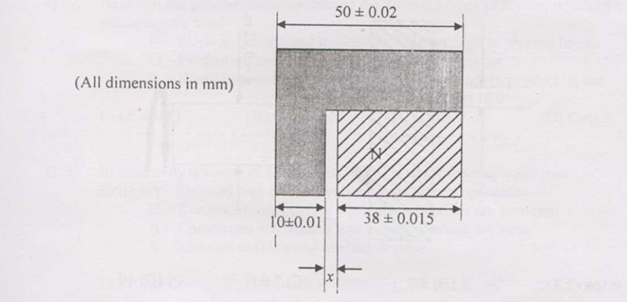
\includegraphics[width=0.5\linewidth]{figs/Q.39.png}
    \caption{fig5}
    \label{fig:figs/Q.39.png}
\end{figure}
       
   \hfill{GATE 2007 PI}
   \begin{enumerate}
   \begin{multicols}{4}
       \item $\pm$ 0.025
       \item $\pm$ 0.030
       \item $\pm$ 0.040
       \item $\pm$ 0.045
       \end{multicols}
\end{enumerate}

\item
The maximum possible percentage reduction in area per pass during wire drawing of an ideal plastic material without friction is of the order of

\hfill{GATE 2007 PI}
\begin{enumerate}
\begin{multicols}{4}
    \item 37
    \item 50
    \item 63
    \item 75
    \end{multicols}
\end{enumerate}

\item 
Circular blanks of 35 mm diameter are punched from a steel sheet of 2 mm thickness. If the clearance per side between the punch and die is to be kept as 40 microns, the sizes of punch and die should respectively be

\hfill{GATE 2007 PI }
\begin{enumerate}
\begin{multicols}{4}
    \item $35^{+0.00}$ and $35^{+0.040}$
    \item $35^{-0.040}$ and $35^{-0.080}$
    \item $35^{+0.00}$ and $35^{+0.080}$
    \item $35^{+0.040}$ and $35^{-0.080}$
    \end{multicols}
\end{enumerate}

\item
In a CAD package, a point $P(6, 3, 2)$ is projected along a vector $v(-2,1,-1 )$. The projection of this point on $X-Y$ plane will be
\hfill{GATE 2007 PI}
\begin{enumerate}
\begin{multicols}{4}
    \item (4,4,0)
    \item (8,2,0)
    \item (7,4,0)
    \item (2,5,0)
    \end{multicols}
\end{enumerate}

\item
The geometric transformation specified by [X'Y'1] = [X Y 1]
 $\begin{bmatrix}
0.5 & 0 & 0 \\
0 & 0.25 & 0 \\
1 & 2 & 1
\end{bmatrix}$ in a 2D CAD system represents

\hfill{GATE 20007 PI}
\begin{enumerate}
\begin{multicols}{2}
    \item scaling and Translation
    \item Scaling and Rotataion
    \item Rotation and Translation
    \item Rotation
    \end{multicols}
\end{enumerate}
\item    
The figure below shows the cross-section of circular fillet weld joining a cylindrical steel pin to a steel plate. If the pin is subjected to a pure torsional load, the shear stress (MPa) occurring at the throat of the weld is


    \begin{figure}[H]
        \centering
        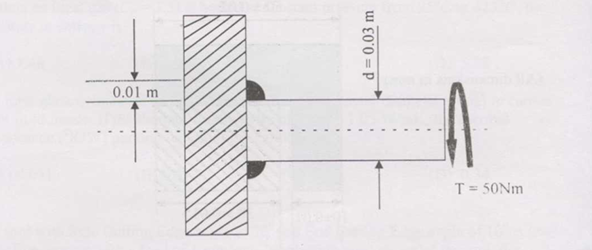
\includegraphics[width=0.5\linewidth]{figs/Q.44.png}
        \caption{fig6}
        \label{fig:figs/Q.44.png}
    \end{figure}
\begin{enumerate}
\begin{multicols}{4}
    \item 2.5
    \item 5.0
    \item 7.0
    \item 10
    \end{multicols}
\end{enumerate}

\item 
 Diameter of a hole after plating needs to be controlled between$30^{+0.050}_{+0.010} \ \text{mm.}$ If the plating thickness varies between 10-15 microns, diameter of the hole before plating should be


 \hfill{GATE 2007 PI}
\begin{enumerate}
\begin{multicols}{4}
    \item $30^{+0.070}_{+0.030} \ \text{mm}$
    \item $30^{+0.065}_{+0.020} \ \text{mm}$
    \item $30^{+0.080}_{+0.030} \ \text{mm}$
    \item $30^{+0.070}_{+0.040} \ \text{mm}$
    \end{multicols}
\end{enumerate}
\item 
The D.C. power source for arc welding has the characteristic 3 V + I = 240, where V = Voltage and I = Current in amp. For maximum arc power at the electrode, voltage should be set at

\hfill{GATE 2007 PI}
\begin{enumerate}
\begin{multicols}{4}
    \item 20 V
    \item 40 V
    \item 60 V
    \item 80 V
    \end{multicols}
    
\end{enumerate}

\item	
In a CNC machine feed drive, a stepper motor with step angle of  $1.8^\circ$
 drives a lead screw with pitch of 2 mm. The Basic Length Unit (BLU) for this drive iS
 
 \hfill{GATE 2007 PI}
 \begin{enumerate}
 \begin{multicols}{4}
     \item 10 microns
     \item 20 microns
     \item 40 microns
     \item 100 microns
     \end{multicols}
 \end{enumerate}
 
\item
 Which one of the following gear manufacturing processes is NOT based on generation principle?

 \hfill{GATE 2007 PI}
 \begin{enumerate}
 \begin{multicols}{4}
     \item Gear Hobbing
     \item Gear Shaping
     \item Gear Milling
     \item Gear Shaving
     \end{multicols}
 \end{enumerate} 

\item
Based on the general characteristics of the different types of layout, which of the following are true?\\
P-Work-in-process and throughput time are high in process layout\\

Q-Constraints are binding when shadow prices are non-zero \\

R-Constraints are binding when shadow prices are zero \\ 

\hfill{GATE 2007 PI}
\begin{enumerate}
\begin{multicols}{4}
    \item P and Q
    \item Q and R
    \item only P
    \item only R
    \end{multicols}
\end{enumerate}

\item
In sensitivity analysis of LP models, which of the following holds true?\\
P-Reduced cost of basic variables are zero at optimality\\

  Q-Constraints are binding when shadow prices are non-zero\\
  
  R-Constraints are binding when shadow prices are zero\\
  
  S-Reduced cost is same as shadow price

  \hfill{GATE 2007 PI}
  \begin{enumerate}
  \begin{multicols}{4}
      \item P and Q
      \item Q and R
      \item P and R
      \item Q and S
      \end{multicols}
  \end{enumerate}
  
  \item 
  Consider the symmetric dual pair of LPs [P] and [D], where $A$ is an $m \times n$ matrix, 
$b$ is an $m$-vector and $c$ is an $n$-vector.

\[
\begin{array}{c|c}
\text{[P] } \min & c^T x \\ 
\text{s.t.} & Ax \ge b \\
& x \ge 0
\end{array}
\quad
\begin{array}{c|c}
\text{[D] } \max & b^T y \\ 
\text{s.t.} & A^T y \le c \\
& y \ge 0
\end{array}
\]

Assume that [P] is feasible. If the optimal values are $z_1^*$ for [P] and $z_2^*$ for [D], 
whenever they exist, then which one of the following is true?

\hfill{GATE 2007 PI}

\begin{enumerate}
\begin{multicols}{2}
    \item If [D] is infeasible, then $z_1^*$ can be determined and is equal to $z_2^*$.
    \item If [D] is feasible, then $z_1^*$ cannot be determined.
    \item If [D] is feasible, then $z_1^*$ can be determined and is equal to $z_2^*$.
    \item If [D] is feasible, then $z_1^*$ can be determined but not equal to $z_2^*$.
    \end{multicols}
\end{enumerate}

\item 
The moving average method is to be used for forecasting demand based on $m$ periods of data. 
Two values of $m$ are tried, $m_1$ and $m_2$ with $m_1 > m_2$, to get two different forecasts, 
denoted by $F(t)$ and $G(t)$.  
P -- $F(t)$ has less variability than $G(t)$  

Q -- Forecast error of $F(t)$ is less than that of $G(t)$  

Which of the above statements are true?
\hfill{GATE 2007 PI}
\begin{enumerate}
\begin{multicols}{4}
    \item Only P
    \item Only Q
    \item Both P and Q
    \item Neither P nor Q
    \end{multicols}
    \end{enumerate}
    
    \item 
In an optimization problem, let y be a 0-1 variable and x be a positive real number. Now, the condition that x can take non-zero values only ify = 1 can be modeled using the linear constraint

\hfill{GATE 2007 PI}

\begin{enumerate}
\begin{multicols}{4}
    \item $x \leq My$ \quad (M is a large number)
    \item $x \geq y$
    \item $x \geq My$ \quad (M is a large number)
    \item $xy \geq 0$
    \end{multicols}
\end{enumerate}

\item 
The average number of accidents occurring monthly on an assembly shop floor is 2.
The probability that there will be at least one accident in this month is estimated to be

\hfill{GATE 2007 PI}
\begin{enumerate}
\begin{multicols}{4}
    \item 0.055
    \item 0.456
    \item 0.865
    \item 0.950
    \end{multicols}
\end{enumerate}

\item 
$X_1, \ldots, X_{100}$ are Bernoulli random variables with a probability of success equal to $0.6$.  

By the Central Limit Theorem, the random variable  
\[
Y = \sum_{i=1}^{100} X_i\]
is approximately normally distributed.Then $Y$ has mean and variance respectively equal to \dots

\hfill{GATE 2007 PI}
\begin{enumerate}
\begin{multicols}{4}
    \item 40 and 24
    \item 60 and 24
    \item 40 and 12
    \item 60 and 12
    \end{multicols}
    \end{enumerate}

\item 
Karmarkar's algorithm for Linear Programming

\hfill{GATE 2007 PI}
\begin{enumerate}
\begin{multicols}{2}
    \item moves along different extreme point solutions of the feasible region
    \item enumerates all possible extreme point solutions
    \item divides the feasible region into different parts for function evaluation
    \item generates interior point iterates which converges to the optimum solution
    \end{multicols}
\end{enumerate}

\item 
For a transportation problem that has a feasible solution, the northwest corner rule gives a possible solution which is

\hfill{GATE 2007 PI}
\begin{enumerate}
\begin{multicols}{2}
    \item a basic feasible solution to the problem
    \item a near optimal solution to the problem  
    \item the optimal solution to the problem
    \item one of the many optimal solutions to the problem
    \end{multicols}
    \end{enumerate}
    
   \item
The assignment problem in Linear Programming is also an example of a discrete optimization problem. How many feasible solutions are there to this problem defined on n jobs and n persons?

\hfill{GATE 2007 PI}
\begin{enumerate}
\begin{multicols}{4}
    \item $n^n$
    \item $n(n-1)$
    \item $n^2$
    \item $n!$
    \end{multicols}
\end{enumerate}

\item 
{Matching Exercise:} Choose the correct one out of the alternatives A, B, C, D

\begin{tabular}{|l|l|}
\hline
{Group 1} & \ {Group 2} \\ \hline
P -- Knowledge Based System        & 1 -- responds to queries with reports \\ \hline
Q -- Decision Support System       & 2 -- uses statistical rules of inference \\ \hline R -- Management Information System & 3 -- provides recommendations \\ \hline
S -- Data Mining                   & 4 -- uses reasoning techniques \\ \hline
\end{tabular}

\hfill{GATE 2007 PI}
\begin{enumerate}
\begin{multicols}{4}
    \item P-4, Q-3, R-1, S-2
    \item P-2, Q-3, R-1, S-4
    \item P-4, Q-2, R-3, S-1
    \item P-3, Q-4, R-1, S-2
    \end{multicols}
\end{enumerate}

\item 
A process is to be controlled with standard values $\mu$
 = 15 and $\sigma$
 = 3.6. The sample size is 9. The control limits for the X chart are
 
 \hfill{GATE 2007 PI}
\begin{enumerate}
\begin{multicols}{4}
    \item $15 \pm 10.8$     
    \item $15 \pm 3.6$
    \item $0.4 \pm 10.8$
    \item $0.4 \pm 3.6$
    \end{multicols}
\end{enumerate}

\item 
Item P is made from components Q and R. Item Q, in turn, is made from S and T. The lead times for items P, Q, R, S, and T are 2, 3, 10, 5, and 6 weeks, respectively. The lead time (in weeks) needed to respond to a customer order for item P is

\hfill{GATE 2007 PI}
\begin{enumerate}
\begin{multicols}{4}
    \item 10
    \item 11
    \item 12
    \item 26
    \end{multicols}
\end{enumerate}

\item 
The reliability of an equipment for a time to failure exceeding $t$ is given by  
\[
R(t) = \exp(-\lambda t)
\]  
The mean time to failure (MTTF) for this equipment (in hours) is
\hfill{GATE 2007 PI}
\begin{enumerate}
\begin{multicols}{4}
    \item $\lambda$
    \item $\frac{1}{\lambda}$
    \item $\frac{1}{\lambda^2}$
    \item $\lambda^2$
    \end{multicols}
\end{enumerate}

\item 
Four jobs have to be sequenced on a single facility, with the objective of minimizing 
the maximum tardiness 
\[
\max_i \left| \text{Completion time}_i - \text{Due date}_i \right|.
\]
The jobs have due dates and processing times as follows:

\begin{center}
\begin{tabular}{|c|c|c|}
\hline
{Job} & {Due date (day number)} & {Processing time (days)} \\
\hline
P & 5 & 2 \\
Q & 6 & 10 \\
R & 3 & 3 \\
S & 7 & 4 \\
\hline
\end{tabular}
\end{center}

The last job that should be taken up is
\hfill{GATE 2007 PI}
\begin{enumerate}
\begin{multicols}{4}
    \item P
    \item Q
    \item R
    \item S
    \end{multicols}
\end{enumerate}

\item 
An asset investment is made for Rs. 1,20,000. The uniform costs per year are Rs. 40,000 in operating the asset. Uniform benefits per year are either Rs. 60,000 or Rs. 80,000, judged to be equally likely. What is the expected payback period?
\hfill{GATE 2007 PI}
\begin{enumerate}
\begin{multicols}{4}
    \item 3
    \item 4.5
    \item 6
    \item 9
    \end{multicols}
\end{enumerate}
\item 
\begin{center}
\begin{tabular}{|l|c|}
\hline
{Activity} & {Time (minutes)} \\
\hline
machine loading + unloading & 2 \\
machining & 4 \\
walking from one machine to the next & 1 \\
\hline
\end{tabular}
\end{center}

For the data given above, how many machines can be assigned to an operator to minimize 
idle time of the operator and machines?
\hfill{GATE 2007 PI}
\begin{enumerate}
\begin{multicols}{4}
    \item 1
    \item 2
    \item 3
    \item 4
    \end{multicols}
    \end{enumerate}
    
    \item  
    Given \\ 
{Assertion [a]}: Value engineering of a new product is to be done after the original 
design concept is nearly ready for release for manufacture. \\[4pt]
{Reason [r]}: Value engineering aims at reducing the cost of manufacture of a new product.

\hfill{GATE 2007 PI}
\begin{enumerate}
\begin{multicols}{2}
    \item Both [a] and [r] are true and [r] is the correct reason for [a]
    \item Both [a] and [r] are true, but [r] is not the correct reason for [a]
    \item Both [a] and [r] are false
    \item [a] is true but [r] is false
    \end{multicols}
\end{enumerate}

\item  
Given \\ 
{Assertion [a]}: There is a continuous reduction of life cycles of modern day products \\
{Reason [r]}: Product life cycle management reduces to a large extent the new product development time from concept to production \\[4pt]

\hfill{GATE 2007 PI}

\begin{enumerate}
\begin{multicols}{2}
    \item Both [a] and [r] are true and [r] is the correct reason for [a]
    \item Both [a] and [r] are true, but [r] is not the correct reason for [a]
    \item Both [a] and [r] are false
    \item [a] is true but [r] is false
    \end{multicols}
\end{enumerate}

\item 
The problem of finding the rectangle of maximum area with perimeter equal to 20 
can be posed as the constrained optimization problem

\[
\begin{aligned}
&\text{Max} && xy \\
&\text{s.t.} && 2x + 2y = 20 \\
& && x, y \geq 0
\end{aligned}
\]

The solution to this problem is \( x = y = 5 \). 
What is the value of the Lagrange multiplier corresponding to the perimeter constraint?

\hfill{GATE 2007 PI}

\begin{enumerate}
\begin{multicols}{4}
    \item 2.5
    \item 5
    \item 7.5
    \item 10
    \end{multicols}
\end{enumerate}

\item 
A manufacturing system with a production rate p units/day experiences a demand rate of d units/day where p > d. Let Q be the maximum production quantity per period. When the total production in a period reaches Q units, the production is stopped and restarted only when inventory becomes zero. In such a scenario, the maximum cycle inventory is
\hfill{GATE 2007 PI}
\begin{enumerate}
\begin{multicols}{4}
    \item \( Q \cdot p \cdot (p - d) \)
    \item \( \frac{Q}{(p - d)^p} \)
    \item \( \frac{Q}{p} (p - d) \)
    \item \( \frac{p(p - d)}{Q} \)
    \end{multicols}
\end{enumerate}

\item 
In a time study, the observed times and ratings for an elemental operation are as shown below:

\begin{center}
\begin{tabular}{|c|c|c|}
\hline
 & {Reading 1} & {Reading 2} \\
\hline
{Rating (\%)} & 80 & 100 \\
\hline
{Observed time (minutes)} & 0.60 & 0.50 \\
\hline
\end{tabular}
\end{center}

Considering an allowance of 10\% of the normal time, the standard time (in minutes) for the operation is:

\hfill{GATE 2007 PI}

\begin{enumerate}
\begin{multicols}{4}
    \item 0.49
    \item 0.54
    \item 0.98
    \item 1.08
    \end{multicols}
\end{enumerate}

{Common Data questions}\\
{Common Data for questions 71,72,73:}\\
The figure below illustrates a project network describing the precedence relationships among different activities (A-J). The activities along with their duration in weeks are represented as arcs, and the events are shown as nodes (l is the start event and 9 is the end event).


\begin{figure}[H]
    \centering
    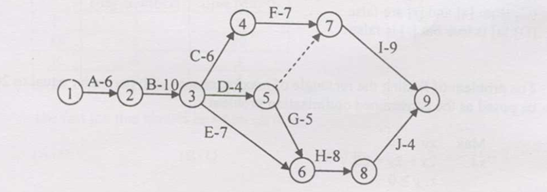
\includegraphics[width=1\linewidth]{figs/Q.71.png}
    \caption{fig7}
    \label{fig:figs/Q.71.png}
\end{figure}
    
    
    \item 
    The length of the crucial path in weeks is
    \hfill{GATE 2007 PI}
    \begin{enumerate}
    \begin{multicols}{4}
        \item 29
        \item 31
        \item 38
        \item 66
        \end{multicols}
    \end{enumerate}
    
    \item 
    If $U_{\alpha}$ is the earliest start time of event $\alpha$, then the reccurence equation defining $U_{6}$
    
    \hfill{GATE 2007 PI}
    \begin{enumerate}
    \begin{multicols}{2}
    \item $U_{6} = \mathrm{Max} \{ U_{8}, 8 \}$
    \item $U_{6} = U_{8} - 8$
    \item $U_{6} = \mathrm{Max} \{ U_{3}, U_{5}, 7, 5 \}$
    \item $U_{6} = \mathrm{Max} \{ U_{3} + 7, U_{5} + 5 \}$
    \end{multicols}
\end{enumerate}

\item 
If activity B has uncertain duration and is uniformly distributed over the interval [8, 12], and T is the earliest start time of event 3 (assume that event I starts at time 0), then the mean and variance of T are
\hfill{GATE 2007 PI}
\begin{enumerate}
\begin{multicols}{4}
    \item 10 and 0.4
    \item 10 and 1.33
    \item 16 and 0.4
    \item 16 and 1.33
    \end{multicols}
    \end{enumerate}
{Common Data for Questions 74,75;}\\
In a Orthogonal machining text, the following observations were made\\
\begin{tabular}{|l|c|}
\hline
{Cutting force} & 1200 N \\ \hline
{Thrust force} & 500 N \\ \hline
{Tool rake angle} & Zero \\ \hline
{Cutting speed} & 1 m/s \\ \hline
{Depth of cut} & 0.8 mm \\ \hline
{Chip thickness} & 1.5 mm \\ \hline
\end{tabular}\\




\item 
Friction angle during machining will be

\hfill{GATE 2007 PI}
\begin{enumerate}
\begin{multicols}{4}
    \item $22.6^{\circ}$
    \item $32.8^{\circ}$
    \item $57.1^{\circ}$
    \item $67.4^{\circ}$
    \end{multicols}
    \end{enumerate}
    
    \item 
    Chip speed along the tool rake face will be
\hfill{GATE 2007 PI}
\begin{enumerate}
\begin{multicols}{4}
    \item 0.83 m/s
    \item 0.53 m/s
    \item 1.2 m/s
    \item 1.88 m/s
    \end{multicols}
    \end{enumerate}
  

    
{Statement for Linked Answer Questions  76 \& 77:}\\
In the setup shown below, $2 \ \mathrm{kW}$ power is supplied by oil flowing into the cylinder of the hydraulic actuator at the rate of $400 \times 10^{-6} \ \mathrm{m}^3/\mathrm{s}$.

    \begin{figure}[H]
        \centering
        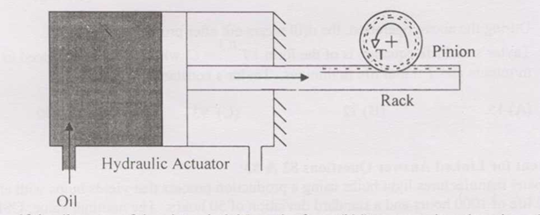
\includegraphics[width=0.5\linewidth]{figs/Q.76.png}
        \caption{fig8}
        \label{fig:figs/Q.76.png}
    \end{figure}
    \item 
    If the diameter of the piston is 0.05 m, the force (kN) generated on the piston is
 
    \hfill{GATE 2007 PI}
    \begin{enumerate}
    \begin{multicols}{4}
        \item 1.6
        \item 4.8
        \item 9.8
        \item 12.2
        \end{multicols}
    \end{enumerate}
    
    \item 
    The pinion is a spur gear having 30 teeth of 2mm module. The torque T(Nm)
    
    \hfill{GATE 2007 PI}
    \begin{enumerate}
    \begin{multicols}{4}
        \item 1.7
        \item 4.0
        \item 6.8
        \item 8.6
        \end{multicols}
        \end{enumerate}
        {statement for Linked Answer Questions 78 \& 79}\\
        Consider an unbalanced serial assembly line consisting of three workstations that produces a single part. 
The part visits each workstation exactly once. 
The number of parallel machines at each workstation and the processing time at a machine is shown below:

\begin{center}
\begin{tabular}{|c|c|c|}
\hline
{Workstation} & {Number of machines} & {Processing time (minutes)} \\ \hline
1 & 1 & 2 \\ \hline
2 & 2 & 5 \\ \hline
3 & 6 & 10 \\ \hline
\end{tabular}
\end{center}


\item 
What is the capcity (in parts/minute) of the above assembly line?

\hfill{GATE 2007 PI}
\begin{enumerate}
\begin{multicols}{4}
    \item 0.1
    \item 0.4
    \item 0.5
    \item 0.6
    \end{multicols}
\end{enumerate}

\item 
The minimum WIP level that allows the line to operate under maximum capacity is 

\hfill{GATE 2007 PI}
\begin{enumerate}
\begin{multicols}{4}
    \item 1.7
    \item 4.0
    \item 6.8
    \item 8.6
    \end{multicols}
    \end{enumerate}
    {statement for Linked Answer Questions 80 \& 81}\\
    
    Blind holes 10 mm diameter, 50 mm deep are being drilled in steel block. Drilling spindle speed is 600 rpm, feed 0.2 mm/rev, Point angle of drill is $120^{\circ}$.\\
    
    
    \item 
    Machining time (in minutes) per hole will be

    \hfill{GTAE 2007 PI}
\begin{enumerate}
\begin{multicols}{4}
    \item 0.08
    \item 0.31
    \item 0.44
    \item 0.86
    \end{multicols}
    \end{enumerate}
    
    \item 
    During the above operation, the drill wears out after producing 200 holes. Taylor's tool life equation is ofthe form $VT^{0.3}$
 = C, V = cutting speed in miminute and T = tool life in minutes. Taylor's constant C will be
    \hfill{GATE 2007 PI}
    \begin{enumerate}
    \begin{multicols}{4}
        \item 15
        \item 72
        \item 93
        \item 490
        \end{multicols}
        \end{enumerate}
        {Statement for Linked Answer Questions  82 \& 83:}\\
        
        A company manufactures light bulbs using a production process that yields bulbs with an average life of 1000 hours and a standard deviation of 50 hours. The nominal value, USL and LSL are 1100 hours, 1300 hours, and 900 hours respectively.\\
        
        
        \item 
        The process capability index $(C_{pk})$ for the manufacturing process is
        
\hfill{GATE 2007 PI}
\begin{enumerate}
\begin{multicols}{4}
    \item 0.67
    \item 1.00
    \item 1.33
    \item 2.00
    \end{multicols}
    \end{enumerate}
    
    \item 
 For the above manufacturing process, the ratio of the potential process capability to its actual process capability is
 
 \hfill{GATE 2007 PI}
 \begin{enumerate}
 \begin{multicols}{4}
     \item 0.50
     \item 0.67
     \item 1.00
     \item 2.00
     \end{multicols}
 \end{enumerate}
 {Statement for Linked Answer Questions 84 \& 85:}\\
 
 In a sand casting process, a sprue of 10 mm base diameter and 250 mm height leads to a runner which fills a cubical mould cavity of 100 mm size\\
 
 
\item 
The volume flow rate (in $\mathrm{mm}^3/\mathrm{s}$
)
\hfill{GATE 2007 PI}
\begin{enumerate}
\begin{multicols}{4}
\item $0.8 \times 10^{5}$
\item $1.1 \times 10^{5}$
\item $1.7 \times 10^{5}$
\item $2.3 \times 10^{5}$
\end{multicols}
\end{enumerate}

\item 
The mould filling time (in seconds) is
\hfill{GATE 2007 PI}
\begin{enumerate}
\begin{multicols}{4}
    \item 2.8
    \item 5.78
    \item 7.54
    \item 8.41
    \end{multicols}
\end{enumerate}


.
   





\end{enumerate}

\end{document}











\end{document}


\end{document}




                        
                    
                        
                    
                
        
                  
                

                


            





     
      
    



\end{document}  